\chapter{Discussion} \label{Chap5} % NEED ALGORITHM DiSCUSSION WHICH SUITABLE FOR LAYOUT, CHECK FOR CHAT, and TURNITIN
\section{Time Complexity}
\subsection{Interaction Mapping Layout} % done chat
The \lstinline{InteractionMapping} algorithm, particularly the \mycode{calculate\_final\_maps} method, can be computationally intensive, especially in the worst-case scenario. During its execution, several key operations contribute to its complexity. Initially, the algorithm performs pre-processing steps, such as generating the \acrfull{qpi} matrix and calculating logical priorities and physical connectivity. These steps run in polynomial time relative to the number of physical qubits and two-qubit operations in the \acrshort{dag}. However, the main challenge arises in the core loop of the \mycode{calculate\_final\_maps} function, where the algorithm iteratively assigns logical qubits to physical qubits. \\
During this process, the algorithm checks and updates possible mappings in a \mycode{while logical\_priority} loop, which continue until all logical qubits are assigned. Each iteration may create several new mappings, causing the number of possibilities to increase exponentially, as the algorithm must consider at a rate of $O(2^k \times |P|)$, where $k$ is the recursion depth and $|P|$ is the number of physical qubits. As a result, the overall time complexity in the worst case is \textbf{exponential}, potentially reaching $O(2^k \times |P| \times n)$, where $n$ is the number of logical qubits. This exponential growth is due to the combinatorial nature of the problem, where multiple candidate mappings are explored and expanded. In practical implementations, this could result in significant computational overhead as the number of qubits increases.

\subsection{Lookahead Swap Routing} % done chat
The \lstinline{DynamicLookaheadSwap} algorithm is a heuristic method designed to map logical qubits to physical qubits in quantum circuits, especially on hardware with limited connectivity. The goal of the algorithm is to reduce the number of additional swap gates required when implementing the circuit on the target hardware, consequently, reducing the circuit depth as well. \\
The algorithm begins with an initialization phase, where it preprocesses the quantum circuit and sets up necessary data structures. This phase runs in linear time proportional to the number of gates. The algorithm then categorizes and analyzes dependencies between gates, focusing on two-qubit operations. This step is also a linear time complexity of $O(G)$, where $G$ is the total number of two-qubit gates in the \acrshort{dag}. \\
In the main loop, the algorithm iterates over each layer of the circuit and checks whether the current qubit layout allows direct execution of two-qubit gates or if a swap operation is necessary. This \mycode{check\_gate\_connectivity} has a time complexity of $O(G \times n^2)$, where $n$ is the number of qubits. The algorithm then \mycode{generate\_possible\_swaps} operations by considering the neighbours of the involved qubits in the coupling map, with a complexity of $O(G \times n^2 \times D)$, where $D$ is the degree of connectivity in the coupling map. \\
For each potential swap, the algorithm evaluates its effect on the circuit using the \mycode{sum\_effect} method. This method assesses how the swap improves qubit placement for future gates by exchanging physical qubits and reducing the distance between qubits. This swap evaluation process can be computationally intensive, with a worst-case time complexity of $O(S \times G)$, where $S$ is the number of candidate swaps. If a beneficial swap is identified, it is applied to the layout at $O(1)$, which further modifies the circuit structure. \\
Overall, the worst-case time complexity of the \lstinline{DynamicLookaheadSwap} algorithm is approximately $O(G \times n^2 \times D + S \times G)$, reflecting the number of two-qubit gates, qubits, and the connectivity of the coupling map. Despite the potential for high computational costs, the algorithm's use of heuristics and the pruning of less beneficial swaps helps manage its complexity, making it a practical approach for optimizing quantum circuits on devices with limited qubit connectivity.

\section{Coupling Graph Options} % done chat
\subsection{Choosing Layout}
The algorithm tested involves around 20 qubits, which aligns with previous studies \cite{li_tackling_2019, zhu_dynamic_2020} that used 5 to 20 qubits in quantum programs sourced from IBM Qiskit \cite{siraichi_qubit_2018, zulehner_efficient_2018} and RevLib \cite{wille_revlib_2008}. The chosen layout configurations-\textit{full}, \textit{grid}, \textit{ring}, \textit{t\_horizontal}, and \textit{t\_vertical}-were selected to determine which layout offers the best performance based on node connectivity. The \textit{t\_horizontal} and \textit{t\_vertical} layouts, derived from a 5-qubit T-shaped IBM backend, were specifically tested to assess how the chain's length at either end impacts qubit mapping performance. \\
When analyzing the distribution of additional swap gates, the \textit{full} layout consistently outperforms the \textit{grid} and \textit{ring} layouts. Full connectivity allows any qubit to interact directly with any other qubit, eliminating the need for intermediate swaps and ensuring the shortest path between qubits is always direct \cite{hayes_graph_2000}. The \textit{grid} layout ranks second, as it has several nodes with three neighbours, compared to the \textit{ring} layout, where each node has only two neighbours. The \textit{grid} layout requires additional operations to manage qubit connectivity, and the \textit{ring} layout structure further limits efficient algorithm implementation, leading to higher resource use and less efficient computation \cite{peham_optimal_2023}. The \textit{t\_horizontal\_5\_4} and \textit{t\_vertical\_5\_4} layouts show no significant difference in additional swap gates and are similar to the \textit{line\_20\_1} layout, indicating they share a linear arrangement. In summary, the number of neighbouring qubits significantly impacts the reduction of additional swap gates needed. An illustration of how logical qubits are placed on physical qubits is provided in Appendix \ref{app:virtual-on-physical-illustration}. \\
Surprisingly, the \textit{grid} layout proved to be the most stable in terms of circuit depth, successfully running all algorithms compared to the \textit{full} and \textit{ring} layouts. The \textit{t\_horizontal} and \textit{t\_vertical} layouts also performed well, running all 15 algorithms. This stability likely stems from the presence of qubits with three neighbours in these layouts, which enhances their ability to handle circuit depth effectively. Although \textit{t\_horizontal\_5\_4} and \textit{t\_vertical\_5\_4} performed similarly to \textit{line\_20\_1} in terms of additional swap gates, they exhibited slightly higher variance in circuit depth. The \lstinline{LookaheadSwap} algorithm works well with these three layouts because it prioritizes executing as many active gates as possible from the dependency list while performing SWAP operations simultaneously \cite{zhang_depth_2020}. In contrast, the \textit{ring} layout is limited by its linear qubit configuration, and the \textit{full} layout struggles with large traversal nodes when evaluating swap candidates. This suggests that an optimal number of neighbouring qubits - neither too many nor too few - is necessary to maintain a balanced circuit depth when using Algorithm \ref{alg:interaction-layout-mapping} \mycode{InteractionLayoutMapping}. \\
\subsection{Choosing Number of Groups}
According to the results shown in Figure \ref{fig:chart-box-plot-group-all}, Group 2 outperformed the other groups with low variability. This success is attributed to dividing tasks into fewer groups, which reduces the number of communication channels required between groups. With only two groups, communication overhead is minimized, as there is only one direct communication link, simplifying data exchange and reducing potential bottlenecks from waiting on other groups \cite{cuomo_optimized_2023}. In contrast, increasing the number of groups complicates coordination, requiring more complex synchronization and qubit allocation across groups \cite{cicconetti_resource_2022}. This added complexity can introduce overhead in the initial qubit mapping, as seen in the failed interaction mapping for the \textit{full\_5\_4} layout. Fewer groups result in simpler coordination, fewer dependencies to manage, and less overall system complexity. \\
In the context of networked quantum computers, it is still crucial to maintain high connectivity within the individual quantum computers inside each group. Even as tasks are divided to reduce inter-group communication overhead, the internal connectivity of each quantum computer must remain robust to ensure efficient qubit interactions. High connectivity within a quantum computer allows for more flexible and efficient execution of quantum operations, minimizing the need for additional swap gates and reducing circuit depth. This balance between minimizing communication overhead across groups and maintaining strong internal connectivity is key to optimizing the overall performance of quantum networks.

% NEED ALGORITHM DISCUSSION !!!!! compare and contrast?

\section{Limitation and Errors} % done chat
Appendix \ref{app:failed-algorithm-layout} details the layouts where timeouts occurred during quantum circuit transpilation. The \lstinline{InteractionMapping} algorithm generally succeeds in mapping logical to physical qubits, except for the \textit{full\_5\_4} layout, where it failed due to a timeout during qubit placement. This issue arises because the algorithm, when traversing possible neighbours, encounters an excessively large tree. To address this, the algorithm includes an exit function that checks if the coupling map is fully connected by calculating the number of neighbours for each physical qubit. If more than 80\% of physical qubits have the maximum number of neighbours, the algorithm exits early and returns a one-to-one mapping. For example, in the best case, the \textit{full\_10\_2} layout has 9 neighbours for 18 qubits and 10 neighbours for 2 qubits that connecting groups, allowing the algorithm to detect the full connectivity and return the one-to-one mapping quickly. However, the \textit{full\_5\_4} layout, with 4 neighbours for 14 qubits and 5 neighbours for 6 qubits, fails to meet the 80\% threshold, causing the algorithm to continue exploring all possibilities until it runs out of memory. A suggested solution to overcome this problem is to analyze the local graph characteristics and check if the graph is $k$-connected \cite{cornejo_connectivity_2010}. \\
Similarly, the \lstinline{LookaheadSwap} algorithm generally works well but begins to fail for certain algorithms at a circuit size of 10 in the \textit{ring\_7\_3} and \textit{ring\_5\_4} layouts, and at a circuit size of 15 in the \textit{full\_7\_3} layout, as well as the previous two layouts. The swap timeout error likely occurs due to the greedy nature of the qubit placement, which assigns logical qubits to the physical qubits with the highest connectivity. In ring layouts, the algorithm starts mapping from the center and branches out. If there are multiple active gates, the algorithm may direct one gate to a branch end but still fail to find adjacent physical qubits to operate the gate, leading to an infinite loop between two nodes at the end until timeout, as illustrated in Figure \ref{fig:swap-stuck}. One strategy to address this issue is to keep an empty list to track assigned physical qubits, but this can cause problems when multiple gates are active. If one gate completes, the next might get stuck because the necessary qubits to go back are already assigned. A potential solution could involve allowing the algorithm to backtrack to certain points in the layout and explore alternative paths \cite{parizek_fast_2019}.
\begin{figure}
    \centering
    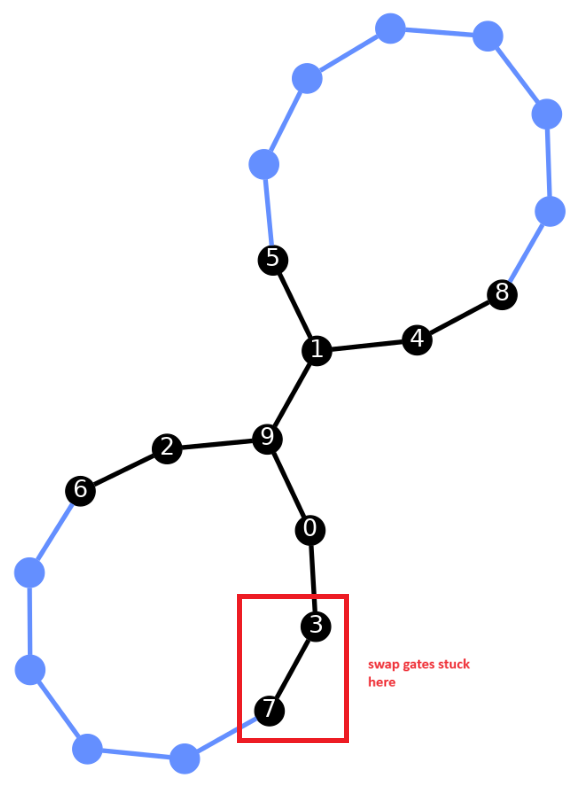
\includegraphics[width=0.5\linewidth]{image/swap_stuck.png}
    \caption{The swap operation is stuck because the highest Lookahead value is at $Q_7$ and $Q_3$.}
    \label{fig:swap-stuck}
\end{figure}

\section{Direction of Future Work} % done chat
This section outlines potential future enhancements to optimize the current algorithm:
\begin{enumerate}[nolistsep]
    \item \textbf{Incorporating Noise}: The current work assumes quantum devices without noise. However, in practice, the noise levels can vary between physical qubits on the same device, which should be factored into the algorithm \cite{niu_hardware_2020}. Future work could integrate noise considerations by configuring constraints, instruction sets, qubit properties, operation timing, and other parameters using the IBM \lstinline{Target} \cite{ibmquantum_target} class.
    \item \textbf{Addressing Communication Costs in Distributed \acrshort{qpu}}: The current approach does not account for the communication cost between groups in a distributed \acrshort{qpu}. Communication between distant quantum computers can introduce higher noise and errors, affecting gate fidelity and disrupting entanglement \cite{murali_noise_adaptive_2019}. Future work could incorporate communication costs into the initial qubit mapping process \cite{houshmand_evolutionary_2020}, either by evenly distributing logical qubits when communication costs are low or by grouping them locally when communication costs are high.
    \item \textbf{Unidirectional Connectivity Constraints}: The coupling graph used in this work assumes bidirectional connections, where two-qubit gates can operate in both directions. A future enhancement could involve considering unidirectional connectivity constraints, which are more restrictive, and refining the search strategy to improve performance under these conditions \cite{sanaei_one_2019}.
    \item \textbf{Utilizing Optimization Techniques}: Currently, the algorithm only calculates the difference in additional swap gates before and after transpilation. Future work could introduce additional optimization stages, such as applying passes that check gate commutation rules \cite{itoko_quantum_2019} and optimizing gate decomposition \cite{rudolph_decomposition_2024}, to further enhance performance.
\end{enumerate}